%%%%%%%%%%%%%%%%%%%%%%%%%%%%%%%%%%%%%%%%%%%%%%%%%%%%%%%%%%%%%
%% Rotating field theory %%
%%%%%%%%%%%%%%%%%%%%%%%%%%%%%%%%%%%%%%%%%%%%%%%%%%%%%%%%%%%%%
\section{Rotating field theory}


%%%%%%%%%%%%%%%%%%%%%%%%%%%%%%%%%%%%%%%%%%%%%%%%%%%%%%%%%%%%%
%% Conceptual idea of a rotating magnetic field %%
%%%%%%%%%%%%%%%%%%%%%%%%%%%%%%%%%%%%%%%%%%%%%%%%%%%%%%%%%%%%%
\begin{frame}
	\frametitle{Conceptual idea of a rotating magnetic field}
    \begin{figure}
        \centering
        \movie{\includegraphics[height=0.7\textheight]{fig/lec05/Three_phase_coils_rotating_field_preview.png}}{fig/lec05/Three_phase_coils_rotating_field.gif}
        \caption{Animation of a rotating magnetic field produced by three-phase currents in three coils both physically and electrically displaced by $120^\circ$ (inspired by \href{https://perso.univ-lyon1.fr/charles.joubert/web_anim/simen_rotfield_create.html}{C.~Joubert})}
        \label{fig:Three_phase_coils_rotating_field_animation}
    \end{figure}
\end{frame}

%%%%%%%%%%%%%%%%%%%%%%%%%%%%%%%%%%%%%%%%%%%%%%%%%%%%%%%%%%%%%
%% MMF distribution of a single-phase coil %%
%%%%%%%%%%%%%%%%%%%%%%%%%%%%%%%%%%%%%%%%%%%%%%%%%%%%%%%%%%%%%
\begin{frame}
	\frametitle{MMF distribution of a single-phase coil}
    \begin{figure}
            \centering
            \includegraphics[width=0.8\textwidth]{fig/lec05/MMF_single_phase.pdf}
            \caption{MMF of a lumped single-phase coil with $N$ turns for some current $i_\mathrm{a} \neq 0$ with the rotating integration path $\partial S$  along the circumference coordinate $\vartheta$. The rotor is considered an unspecific solid iron dummy. Both stator and iron have infinite magnetic permeability.}
            \label{fig: MMF_single_phase}
    \end{figure}
\end{frame}

%%%%%%%%%%%%%%%%%%%%%%%%%%%%%%%%%%%%%%%%%%%%%%%%%%%%%%%%%%%%%
%% MMF distribution of a single-phase coil %%
%%%%%%%%%%%%%%%%%%%%%%%%%%%%%%%%%%%%%%%%%%%%%%%%%%%%%%%%%%%%%
\begin{frame}
	\frametitle{MMF distribution of a single-phase coil (cont.)}
    \onslide<1->
			Utilizing Amp\`ere's law in the magnetic network context from \eqref{eq:ampere_law_magnetic_network}
            $$ \oint_{\partial S} \bm{H} \cdot \mathrm{d}\bm{s} = i_{\mathrm{f}} = N i = \sum_k  \theta_k = \sum_k l_k H_k $$ \onslide<2->
            and assuming that the air gap path along $\delta$ is dominating the magnetic circuit, we have
            \begin{equation}
                H_\mathrm{a}(\vartheta) = \frac{1}{2\delta} \theta_\mathrm{a}(\vartheta) = \frac{1}{2\delta} \begin{cases}
                    N i_\mathrm{a} & \text{for } -\pi/2 \leq \vartheta < \pi/2, \\
                    -N i_\mathrm{a} & \text{for } \pi/2 \leq \vartheta < 3\pi/2.
                \end{cases}
            \end{equation}
            \onslide<1->
            \begin{figure}
                \centering
                \includegraphics[width=0.5\textwidth]{fig/lec05/MMF_single_phase.pdf}
            \end{figure}
\end{frame}

%%%%%%%%%%%%%%%%%%%%%%%%%%%%%%%%%%%%%%%%%%%%%%%%%%%%%%%%%%%%%
%% Air gap flux density distribution of a single-phase coil %%
%%%%%%%%%%%%%%%%%%%%%%%%%%%%%%%%%%%%%%%%%%%%%%%%%%%%%%%%%%%%%
\begin{frame}
	\frametitle{Air gap flux density distribution of a single-phase coil}
    With $B=\mu_0 H$ in the air gap and an alternating current $i_\mathrm{a} = i_\mathrm{a}(t)$, we have
    \begin{equation}
        B_\mathrm{a}(\vartheta, t) = \frac{\mu_0}{2\delta} \begin{cases}
            N i_\mathrm{a}(t) & \text{for } -\pi/2 \leq \vartheta < \pi/2, \\
            -N i_\mathrm{a}(t) & \text{for } \pi/2 \leq \vartheta < 3\pi/2.
        \end{cases}
    \end{equation}
    \pause
    \begin{figure}
        \begin{columns}
            \begin{column}{0.7\textwidth}
                \centering
		\begin{subfigure}[b]{0.45\textwidth}
			\centering
			\includegraphics[width=\textwidth]{fig/lec05/B_single_phase_full_current.pdf}
			\caption{$i_\mathrm{a}(t) = \hat{i}$}
		\end{subfigure}
		\hfill
        \pause
		\begin{subfigure}[b]{0.45\textwidth}
			\centering
			\includegraphics[width=\textwidth]{fig/lec05/B_single_phase_half_current.pdf}
			\caption{$i_\mathrm{a}(t) = \hat{i}/2$}
		\end{subfigure}
            \end{column}
            \begin{column}{0.3\textwidth}
                \caption{\raggedright Air gap flux density distribution of a lumped single-phase coil representing a spatiotemperal function together with its fundamental component $B^{(1)}$} 
        \label{fig:Air_gap_flux_density_single_phase_coil}
            \end{column}
        \end{columns}
	\end{figure}
\end{frame}

%%%%%%%%%%%%%%%%%%%%%%%%%%%%%%%%%%%%%%%%%%%%%%%%%%%%%%%%%%%%%
%% Fourier analysis of the air gap flux density distribution %%
%%%%%%%%%%%%%%%%%%%%%%%%%%%%%%%%%%%%%%%%%%%%%%%%%%%%%%%%%%%%%
\begin{frame}
	\frametitle{Fourier analysis of the air gap flux density distribution}
        Assuming a sinusoidal current $i_\mathrm{a}(t) = \hat{i} \cos(\omega t)$, we have
        \begin{equation}
            B_\mathrm{a}(\vartheta, t) = \underbrace{\frac{\mu_0 N \hat{i}}{2\delta}}_{\hat{B}} \begin{cases}
                \cos(\omega t) & \text{for } -\pi/2 \leq \vartheta < \pi/2, \\
                -\cos(\omega t) & \text{for } \pi/2 \leq \vartheta < 3\pi/2.
            \end{cases}
            \label{eq:B_single_phase_coil}
        \end{equation}
        \pause
        The flux density distribution therefore is periodic and has a sinusoidal shape over $t$ as well as a rectangular shape over $\vartheta$. \pause To analyze the latter in terms of its fundamental and harmonic components, we utilize the Fourier series expansion for some arbitrary $t\in\mathbb{R}$:
        \begin{equation}
            B_\mathrm{a}(\vartheta, t) =B_\mathrm{a}(\vartheta) = \hat{B}^{(0)} + \sum_{k=1}^{\infty} \hat{B}_{\mathrm{c}}^{(k)} \cos(k \vartheta) + \hat{B}_{\mathrm{s}}^{(k)} \sin(k \vartheta),
            \label{eq:fourier_series_B_single_phase_coil}
        \end{equation} 
        for harmonic order $k\in\mathbb{N}$ with amplitudes $\hat{B}_{\mathrm{c}}^{(k)}\in\mathbb{R}$ and $\hat{B}_{\mathrm{s}}^{(k)}\in\mathbb{R}$ as well as offset $\hat{B}^{(0)}\in\mathbb{R}$.
\end{frame}

%%%%%%%%%%%%%%%%%%%%%%%%%%%%%%%%%%%%%%%%%%%%%%%%%%%%%%%%%%%%%
%% Fourier analysis of the air gap flux density distribution (cont.) %%
%%%%%%%%%%%%%%%%%%%%%%%%%%%%%%%%%%%%%%%%%%%%%%%%%%%%%%%%%%%%%
\begin{frame}
	\frametitle{Fourier analysis of the air gap flux density distribution (cont.)}
        The coefficients of \eqref{eq:fourier_series_B_single_phase_coil} are
        \begin{equation}
            \begin{split}
                \hat{B}^{(0)} &= \frac{1}{2\pi} \int_{0}^{2\pi} B(\vartheta) \mathrm{d}\vartheta, \\
                \hat{B}_{\mathrm{c}}^{(k)} &= \frac{1}{\pi} \int_{0}^{2 \pi} B(\vartheta) \cos(k \vartheta) \mathrm{d}\vartheta, \\
                \hat{B}_{\mathrm{s}}^{(k)} &= \frac{1}{\pi} \int_{0}^{2\pi} B(\vartheta) \sin(k \vartheta) \mathrm{d}\vartheta.
            \end{split}
        \end{equation}
        \pause
       Since the positive and negative areas under the MMF curve in \figref{fig: MMF_single_phase} are identical in size, the magnetic field does not have any offset component:
        $$\hat{B}^{(0)} = 0.$$ \pause Furthermore, \eqref{eq:B_single_phase_coil} is an even function, i.e., $B(\vartheta)=B(-\vartheta)$ (i.e., the function is mirror-symmetrical to the $\vartheta$ axis -- cf. \figref{fig:Air_gap_flux_density_single_phase_coil}), leading to $$\hat{B}_{\mathrm{s}}^{(k)} = 0.$$
\end{frame}

%%%%%%%%%%%%%%%%%%%%%%%%%%%%%%%%%%%%%%%%%%%%%%%%%%%%%%%%%%%%%
%% Fourier analysis of the air gap flux density distribution (cont.) %%
%%%%%%%%%%%%%%%%%%%%%%%%%%%%%%%%%%%%%%%%%%%%%%%%%%%%%%%%%%%%%
\begin{frame}
	\frametitle{Fourier analysis of the air gap flux density distribution (cont.)}
        \onslide<+-> Finally, \eqref{eq:B_single_phase_coil} is symmetrical w.r.t. the abscissa, i.e., $B(\vartheta)=-B(\vartheta+\pi)$ (mirrored positive and negative half-wave), leading to
        $$\hat{B}_{\mathrm{c}}^{(k)} = 0 \quad \mbox{for } \quad k=2,4,6,\ldots .$$ \onslide<+->
        Summarizing the above, the Fourier series for the air gap flux density boils down to
        \begin{equation}
            B_\mathrm{a}(\vartheta) = \sum_{k=1,3,5,\ldots}^{\infty} \hat{B}_{\mathrm{c}}^{(k)} \cos(k \vartheta) \quad \mbox{with} \quad \hat{B}_{\mathrm{c}}^{(k)} = \frac{1}{\pi} \int_{0}^{2 \pi} B(\vartheta) \cos(k \vartheta) \mathrm{d}\vartheta.
            \label{eq:fourier_series_B_single_phase_coil_reduced}
        \end{equation} \onslide<+->
        Utilizing symmetry of the flux distribution as shown in \figref{fig:Air_gap_flux_density_single_phase_coil}, we can calculate $\hat{B}_{\mathrm{c}}^{(k)}$ for the remaining odd $k=1,3,5,\ldots$ harmonic orders as follows:
        \begin{equation}
            \begin{split}
                \hat{B}_{\mathrm{c}}^{(k)} &= \frac{2}{\pi} \int_{-\pi/2}^{\pi/2} B(\vartheta) \cos(k \vartheta) \mathrm{d}\vartheta =  \uncover<+->{\frac{\mu_0 N \hat{i}}{\delta \pi } \cos(\omega t) \int_{-\pi/2}^{\pi/2} \cos(k \vartheta) \mathrm{d}\vartheta} \\ &\uncover<+->{= \frac{\mu_0 N \hat{i}}{k \delta \pi } \cos(\omega t) \left[ \sin(\frac{k \pi}{2}) - \sin(-\frac{k \pi}{2}) \right]}\uncover<+->{= \frac{2 \mu_0 N \hat{i}}{\delta \pi k} \cos(\omega t) \sin(\frac{k \pi}{2}).}
            \end{split}
            \label{eq:B_single_phase_coil_fourier_series_coefficients}
        \end{equation}
\end{frame}

%%%%%%%%%%%%%%%%%%%%%%%%%%%%%%%%%%%%%%%%%%%%%%%%%%%%%%%%%%%%%
%% Fourier analysis of the air gap flux density distribution (cont.) %%
%%%%%%%%%%%%%%%%%%%%%%%%%%%%%%%%%%%%%%%%%%%%%%%%%%%%%%%%%%%%%
\begin{frame}
	\frametitle{Fourier analysis of the air gap flux density distribution (cont.)}
    \onslide<+-> The Fourier series describing the spatiotemperal air gap flux density distribution of a lumped single-phase coil is therefore
    \begin{equation}
        \begin{split}
            B_\mathrm{a}(\vartheta, t) &= \frac{2 \mu_0 N \hat{i}}{\delta \pi}\cos(\omega t)\sum_{k=1,3,5,\ldots}^{\infty}   \frac{1}{k}\sin(\frac{k \pi}{2}) \cos(k \vartheta)\\ &\uncover<+->{= \frac{4}{\pi} \hat{B} \cos(\omega t)\sum_{k=1,3,5,\ldots}^{\infty}   \frac{1}{k}\sin(\frac{k \pi}{2}) \cos(k \vartheta).}
            \label{eq:B_single_phase_coil_fourier_series}
        \end{split}
    \end{equation}
    \onslide<+->
    One might note that $$\sin(\frac{k \pi}{2}) = 1 \quad \mbox{for } k=1,5,9,\ldots, \qquad \sin(\frac{k \pi}{2}) = -1 \quad \mbox{for } k=3,7,11,\ldots$$ applies above. \onslide<+-> Also, the fundamental component $\hat{B}^{(1)}$ of the air gap flux density distribution is $4/\pi$ times higher than the amplitude $\hat{B}$ of the original square wave function from \eqref{eq:B_single_phase_coil} while the harmonic amplitudes decrease with $1/k$. 
\end{frame}

%%%%%%%%%%%%%%%%%%%%%%%%%%%%%%%%%%%%%%%%%%%%%%%%%%%%%%%%%%%%%
%% Fourier analysis of the air gap flux density distribution (cont.) %%
%%%%%%%%%%%%%%%%%%%%%%%%%%%%%%%%%%%%%%%%%%%%%%%%%%%%%%%%%%%%%
\begin{frame}
	\frametitle{Fourier analysis of the air gap flux density distribution (cont.)}
    \begin{columns}
        \begin{column}{0.6\textwidth}
            \begin{figure}
            \centering
            \includegraphics[width=0.825\textwidth]{fig/lec05/B_single_phase_harmonics.pdf}
            \caption{Decomposition of $B(\vartheta, t)$ for $t=0$ into its fundamental and its first harmonic components}
            \label{fig:B_single_phase_harmonics}
        \end{figure}
        \end{column}
        \pause
        \begin{column}{0.4\textwidth}
            \begin{varblock}{Flux density harmonics}
                The existence of harmonics is to be attributed to the spatial layout of the winding. The phase current was assumed to be of pure sinusoidal form, i.e., is not causing the flux density harmonics (in our investigation).
            \end{varblock}
        \end{column}
    \end{columns}
\end{frame}

%%%%%%%%%%%%%%%%%%%%%%%%%%%%%%%%%%%%%%%%%%%%%%%%%%%%%%%%%%%%%
%% Multipole stators %%
%%%%%%%%%%%%%%%%%%%%%%%%%%%%%%%%%%%%%%%%%%%%%%%%%%%%%%%%%%%%%
\begin{frame}
	\frametitle{Multipole stators}
        \begin{figure}
                \centering
                \includegraphics[width=0.8\textwidth]{fig/lec05/MMF_single_phase_two_pole_pairs.pdf}
                \caption{MMF of a lumped single-phase coil with two pole pairs $p$ and $N/p$ turns per pole pair for some current $i_\mathrm{a} \neq 0$ with the rotating integration path $\partial S$  along the circumference coordinate $\vartheta$}
                \label{fig: MMF_single_phase_two_pole_pairs}
        \end{figure}
\end{frame}

%%%%%%%%%%%%%%%%%%%%%%%%%%%%%%%%%%%%%%%%%%%%%%%%%%%%%%%%%%%%%
%% Multipole stators (cont.) %%
%%%%%%%%%%%%%%%%%%%%%%%%%%%%%%%%%%%%%%%%%%%%%%%%%%%%%%%%%%%%%
\begin{frame}
	\frametitle{Multipole stators (cont.)}
        Following the same derivation as previously for machines with $p\geq 1$ pole pairs, we have    \begin{equation}
            \begin{split}
                B_\mathrm{a}(\vartheta, t) &= \frac{2 \mu_0 N \hat{i}}{\delta \pi p}\cos(\omega t)\sum_{k=1,3,5,\ldots}^{\infty}   \frac{1}{k}\sin(\frac{k \pi}{2}) \cos(k p \vartheta)\\ &= \frac{4}{\pi p} \hat{B} \cos(\omega t)\sum_{k=1,3,5,\ldots}^{\infty}   \frac{1}{k}\sin(\frac{k \pi}{2}) \cos(k p \vartheta).
            \end{split}
            \label{eq:B_single_phase_coil_fourier_series_multi_pole}
        \end{equation}
        \pause
        Compared to the single-pole pair case, the flux density 
        \begin{itemize}
            \item<+-> amplitude is reduced by $1/p$ (due to the winding turns being distributed over $p$ pole pairs),
            \item<+-> spatial frequency is increased by $p$: $\vartheta \rightarrow p \vartheta$. 
        \end{itemize}
        \onslide<+->
        The latter implies that the fundamental and harmonics of $B(\vartheta)$ repeat $p$ times more often over the (mechanical) stator circumference (compare \figref{fig:B_single_phase_harmonics}).
\end{frame}

%%%%%%%%%%%%%%%%%%%%%%%%%%%%%%%%%%%%%%%%%%%%%%%%%%%%%%%%%%%%%
%% Multipole stators (cont.) %%
%%%%%%%%%%%%%%%%%%%%%%%%%%%%%%%%%%%%%%%%%%%%%%%%%%%%%%%%%%%%%
\begin{frame}
	\frametitle{Multipole stators (cont.)}
        From  the previous finding
        \begin{equation*}
                B_\mathrm{a}(\vartheta, t) = \frac{4}{\pi p} \hat{B} \cos(\omega t)\sum_{k=1,3,5,\ldots}^{\infty}   \frac{1}{k}\sin(\frac{k \pi}{2}) \cos(k p \vartheta)
        \end{equation*}
        we can conclude that the field distribution for $p > 1$ is repeated $p$ times over the mechanical stator circumference, assuming that the  machine is ideally identical for each pole pair. 
        \pause
        \begin{varblock}{Electrical vs. mechanical angle}
            To simplify the following analysis, we introduce the electrical angle 
            \begin{equation}
                \vartheta_\mathrm{el} = p \vartheta,
            \end{equation}
           i.e., to complete one mechanical revolution, the electrical angle has to complete $p$ revolutions. The field description in the electrical coordinate system is therefore sufficient, as this is merely repeated in the mechanical system.
        \end{varblock}
\end{frame}

%%%%%%%%%%%%%%%%%%%%%%%%%%%%%%%%%%%%%%%%%%%%%%%%%%%%%%%%%%%%%
%% Basic rotating field model %%
%%%%%%%%%%%%%%%%%%%%%%%%%%%%%%%%%%%%%%%%%%%%%%%%%%%%%%%%%%%%%
\begin{frame}
	\frametitle{Basic rotating field model}
    \begin{columns}
		\begin{column}{0.55\textwidth}
            \onslide<1->
	        We assume an ideal three-phase stator current:
            \begin{equation}
                \begin{split}
                    i_\mathrm{s,a}(t) &= \hat{i}_{\mathrm{s}} \cos(\omega t), \\
                    i_\mathrm{s,b}(t) &= \hat{i}_{\mathrm{s}} \cos(\omega t - 2\pi/3), \\
                    i_\mathrm{s,c}(t) &= \hat{i}_{\mathrm{s}} \cos(\omega t + 2\pi/3).
                \end{split}
            \end{equation}
            \onslide<2->
            The index 's' indicates stator quantities, but is omitted in the following as we will only consider stator quantities until further notice, i.e.,, 
            $$i_\mathrm{s,a}(t) = i_\mathrm{a}(t), \quad i_\mathrm{s,b}(t) = i_\mathrm{b}(t), \quad i_\mathrm{s,c}(t) = i_\mathrm{c}(t)$$
            and $\hat{i}_{\mathrm{s}}=\hat{i}$. 
        \end{column}
        \onslide<1->
        \begin{column}{0.45\textwidth}
            \begin{figure}
                \centering
                \includegraphics[width=0.8\textwidth]{fig/lec05/Simple_three_phase_stator_lumped_coils.pdf}
                \caption{Elementary three-phase stator winding with lumped coils  displaced by $120^\circ$ ($p=1$ pole pair)}
                \label{fig:Simple_three_phase_stator_lumped_coils}
            \end{figure}
        \end{column}
    \end{columns}
\end{frame}

%%%%%%%%%%%%%%%%%%%%%%%%%%%%%%%%%%%%%%%%%%%%%%%%%%%%%%%%%%%%%
%% Basic rotating field model (cont.) %%
%%%%%%%%%%%%%%%%%%%%%%%%%%%%%%%%%%%%%%%%%%%%%%%%%%%%%%%%%%%%%
\begin{frame}
	\frametitle{Basic rotating field model (cont.)}
    \onslide<+->
    Transferring the finding \eqref{eq:B_single_phase_coil_fourier_series_multi_pole} to the three-phase stator winding from \figref{fig:Simple_three_phase_stator_lumped_coils} (considering an arbitrary number of $p \geq 1$ pole pairs), we have
    \begin{equation}
        \begin{split}
            B_\mathrm{a}(\vartheta_\mathrm{el}, t) &= \frac{4}{\pi p} \hat{B} \cos(\omega t)\sum_{k=1,3,5,\ldots}^{\infty}   \frac{1}{k}\sin\left(\frac{k \pi}{2}\right) \cos(k \vartheta_\mathrm{el}),\\
            \uncover<+->{
                B_\mathrm{b}(\vartheta_\mathrm{el}, t) &= \frac{4}{\pi p} \hat{B} \cos\left(\omega t - \frac{2\pi}{3}\right)\sum_{k=1,3,5,\ldots}^{\infty}   \frac{1}{k}\left(\frac{k \pi}{2}\right) \cos\left(k \vartheta_\mathrm{el} - k\frac{2\pi}{3} \right),\\ 
            }
            \uncover<+->{
            B_\mathrm{c}(\vartheta_\mathrm{el}, t) &= \frac{4}{\pi p} \hat{B} \cos\left(\omega t + \frac{2\pi}{3}\right)\sum_{k=1,3,5,\ldots}^{\infty}   \frac{1}{k}\left(\frac{k \pi}{2}\right) \cos\left(k \vartheta_\mathrm{el} +  k \frac{2\pi}{3}\right).
            }
        \end{split}
        \label{eq:B_three_phase_stator_coil_fourier_series}
    \end{equation}
\end{frame}

%%%%%%%%%%%%%%%%%%%%%%%%%%%%%%%%%%%%%%%%%%%%%%%%%%%%%%%%%%%%%
%% Basic rotating field model (cont.) %%
%%%%%%%%%%%%%%%%%%%%%%%%%%%%%%%%%%%%%%%%%%%%%%%%%%%%%%%%%%%%%
\begin{frame}
	\frametitle{Basic rotating field model (cont.)}
    \onslide<+->
    Applying the decomposition $$\cos(x)\cos(y) = \frac{1}{2} \left[ \cos(x-y) + \cos(x+y) \right]$$ to \eqref{eq:B_three_phase_stator_coil_fourier_series}\onslide<2->, we obtain
    \begin{equation*}
        \small
        \begin{split}
            \uncover<+->{
                B_\mathrm{a}(\vartheta_\mathrm{el}, t) &= \frac{2}{\pi p} \hat{B} \sum_{k=1,3,5,\ldots}^{\infty}   \frac{1}{k}\sin\left(\frac{k \pi}{2}\right)\left[\cos(\omega t - k \vartheta_\mathrm{el}) + \cos(\omega t + k \vartheta_\mathrm{el})\right],\\
            }
            \uncover<+->{
            B_\mathrm{b}(\vartheta_\mathrm{el}, t) &= \frac{2}{\pi p} \hat{B} \sum_{k=1,3,5,\ldots}^{\infty}   \frac{1}{k}\sin\left(\frac{k \pi}{2}\right)\left[\cos(\omega t - k \vartheta_\mathrm{el} - \frac{2\pi}{3}(1-k)) + \cos(\omega t + k \vartheta_\mathrm{el} - \frac{2\pi}{3}(1+k))\right],\\
            }
            \uncover<+->{
            B_\mathrm{c}(\vartheta_\mathrm{el}, t) &= \frac{2}{\pi p} \hat{B} \sum_{k=1,3,5,\ldots}^{\infty}   \frac{1}{k}\sin\left(\frac{k \pi}{2}\right)\left[\cos(\omega t - k \vartheta_\mathrm{el} + \frac{2\pi}{3}(1-k)) + \cos(\omega t + k \vartheta_\mathrm{el} + \frac{2\pi}{3}(1+k))\right].
            }
        \end{split}
    \end{equation*}

\end{frame}

%%%%%%%%%%%%%%%%%%%%%%%%%%%%%%%%%%%%%%%%%%%%%%%%%%%%%%%%%%%%%
%% Positive and negative sequence decomposition %%
%%%%%%%%%%%%%%%%%%%%%%%%%%%%%%%%%%%%%%%%%%%%%%%%%%%%%%%%%%%%%
\begin{frame}
	\frametitle{Positive and negative sequence decomposition}
    Hence, the decomposition led to two sinusoidal fields rotating in opposite directions:
    $$\underbrace{\cos(\omega t - k \vartheta_\mathrm{el})=\cos(k \vartheta_\mathrm{el} - \omega t)}_{\mbox{positive sequence}} \qquad  \mbox{and} \qquad \underbrace{\cos(\omega t + k \vartheta_\mathrm{el})}_{\mbox{negative sequence}}.$$
    \begin{figure}
        \centering
        \includegraphics[width=0.9\textwidth]{fig/lec05/Positive_negative_sequence_components.pdf}
        \caption{Decomposition of the alternating field into positive and negative sequence components for $p=1$ and $k=1$}
        \label{fig:Positive_negative_sequence_components}
    \end{figure}
\end{frame}

%%%%%%%%%%%%%%%%%%%%%%%%%%%%%%%%%%%%%%%%%%%%%%%%%%%%%%%%%%%%%
%% Resulting field: positive sequence part %%
%%%%%%%%%%%%%%%%%%%%%%%%%%%%%%%%%%%%%%%%%%%%%%%%%%%%%%%%%%%%%
\begin{frame}
	\frametitle{Resulting field: positive sequence part}
    \onslide<+->
    To describe the resulting field distribution (as visualized in \figref{fig:Three_phase_coils_rotating_field_animation}) 
    \begin{equation}
        B(\vartheta_\mathrm{el}, t) = B_\mathrm{a}(\vartheta_\mathrm{el}, t) + B_\mathrm{b}(\vartheta_\mathrm{el}, t) + B_\mathrm{c}(\vartheta_\mathrm{el}, t)
    \end{equation}
    we analyze the positive and negative sequences separately. \onslide<+-> Utilizing $$\cos(x \pm y) = \cos(x)\cos(y) \mp \sin(x)\sin(y)$$ we obtain for the positive sequence: \onslide<+->
    \begin{equation*}
        \begin{alignedat}{2}
        \uncover<+->{
            &\cos(\omega t - k \vartheta_\mathrm{el}) &&+ \cos(\omega t - k \vartheta_\mathrm{el} - \frac{2\pi}{3}(1-k)) + \cos(\omega t - k \vartheta_\mathrm{el} + \frac{2\pi}{3}(1-k))\\}
        \uncover<+->{
            = \quad &\cos(\omega t - k \vartheta_\mathrm{el}) &&+ \cos(\omega t - k \vartheta_\mathrm{el}) \cos(\frac{2\pi}{3}(1-k)) + \sin(\omega t - k \vartheta_\mathrm{el}) \sin(\frac{2\pi}{3}(1-k))\\
        }
        \uncover<+->{
         & &&+ \cos(\omega t - k \vartheta_\mathrm{el}) \cos(\frac{2\pi}{3}(1-k)) - \sin(\omega t - k \vartheta_\mathrm{el})\sin(\frac{2\pi}{3}(1-k)).   
        }
        \end{alignedat}
    \end{equation*}
    \onslide<+->
    Hence, the sine terms cancel out each other.
\end{frame}


%%%%%%%%%%%%%%%%%%%%%%%%%%%%%%%%%%%%%%%%%%%%%%%%%%%%%%%%%%%%%
%% Resulting field: positive sequence part (cont.) %%
%%%%%%%%%%%%%%%%%%%%%%%%%%%%%%%%%%%%%%%%%%%%%%%%%%%%%%%%%%%%%
\begin{frame}
	\frametitle{Resulting field: positive sequence part (cont.)}
    \onslide<+->
    Summarizing the above, we have
        \begin{align*}
        &\cos(\omega t - k \vartheta_\mathrm{el})  \cos(\omega t - k \vartheta_\mathrm{el} - \frac{2\pi}{3}(1-k)) + \cos(\omega t - k \vartheta_\mathrm{el} + \frac{2\pi}{3}(1-k))\\
         = \quad &\cos(\omega t - k \vartheta_\mathrm{el})(1+2\cos(\frac{2\pi}{3}(1-k))).
    \end{align*}
    \onslide<+->
    Considering $\cos(n 2 \pi)=1$ and $\cos(4\pi/3 + n 2 \pi) = \cos(2\pi/3 + n 2 \pi)=-1/2$ for $n \in \mathbb{Z}$ we observe the following for the positive sequence
    \begin{equation}
        \cos(\omega t - k \vartheta_\mathrm{el})(1+2\cos(\frac{2\pi}{3}(1-k))) = \begin{cases}
            3 \cos(\omega t - k \vartheta_\mathrm{el}) & \text{for } k=1,7,13,19,\ldots, \\
            0 & \text{for } k=3,5,9,11,15, 17,\ldots.
        \end{cases}
    \end{equation}
    \onslide<+->
    Hence, there are multiple harmonic orders which cancel out each other, among others, any multiple of $k=3$. Moreover, the positive sequences of all three phases carries the fundamental component for $k=1$.    
\end{frame}

%%%%%%%%%%%%%%%%%%%%%%%%%%%%%%%%%%%%%%%%%%%%%%%%%%%%%%%%%%%%%
%% Resulting field: negative sequence part %%
%%%%%%%%%%%%%%%%%%%%%%%%%%%%%%%%%%%%%%%%%%%%%%%%%%%%%%%%%%%%%
\begin{frame}
	\frametitle{Resulting field: negative sequence part}
    \onslide<+->
    For the negative sequence part of
    \begin{equation*}
        B(\vartheta_\mathrm{el}, t) = B_\mathrm{a}(\vartheta_\mathrm{el}, t) + B_\mathrm{b}(\vartheta_\mathrm{el}, t) + B_\mathrm{c}(\vartheta_\mathrm{el}, t)
    \end{equation*}
    \onslide<2->
    we rewrite the following terms
    \begin{equation*}
        \begin{alignedat}{2}
        \uncover<+->{    
            &\cos(\omega t + k \vartheta_\mathrm{el}) &&+ \cos(\omega t + k \vartheta_\mathrm{el} - \frac{2\pi}{3}(1+k)) + \cos(\omega t + k \vartheta_\mathrm{el} + \frac{2\pi}{3}(1+k))\\
        }
        \uncover<+->{   
            = \quad &\cos(\omega t + k \vartheta_\mathrm{el}) &&+ \cos(\omega t + k \vartheta_\mathrm{el}) \cos(\frac{2\pi}{3}(1+k)) + \sin(\omega t + k \vartheta_\mathrm{el}) \sin(\frac{2\pi}{3}(1+k))\\
        }
        \uncover<+->{
            & &&+ \cos(\omega t + k \vartheta_\mathrm{el}) \cos(\frac{2\pi}{3}(1+k)) - \sin(\omega t + k \vartheta_\mathrm{el})\sin(\frac{2\pi}{3}(1+k))
        }
        \end{alignedat}
    \end{equation*}
    \onslide<+->
    and find for the negative sequence
    \begin{equation}
        \cos(\omega t + k \vartheta_\mathrm{el})(1+2\cos(\frac{2\pi}{3}(1+k))) = \begin{cases}
            3 \cos(\omega t + k \vartheta_\mathrm{el}) & \text{for } k=5,11,17,\ldots, \\
            0 & \text{for } k=1, 3, 7,9,15, \ldots.
        \end{cases}
    \end{equation}
\end{frame}

%%%%%%%%%%%%%%%%%%%%%%%%%%%%%%%%%%%%%%%%%%%%%%%%%%%%%%%%%%%%%
%% Resulting field: summary %%
%%%%%%%%%%%%%%%%%%%%%%%%%%%%%%%%%%%%%%%%%%%%%%%%%%%%%%%%%%%%%
\begin{frame}
	\frametitle{Resulting field: summary}
    Combining the positive and negative sequences, we receive
    \begin{equation}
        B(\vartheta_\mathrm{el}, t) = \frac{6}{\pi p} \hat{B} \sum_{k}^{\infty} \frac{1}{k} \sin\left(\frac{k \pi}{2}\right) \begin{cases}
            \cos(\omega t - k \vartheta_\mathrm{el}) & \text{for } k=1,7,13,19,\ldots, \\
            \cos(\omega t + k \vartheta_\mathrm{el}) & \text{for } k=5,11,17,\ldots, \\
            0 & \text{otherwise}.
        \end{cases}
    \end{equation}
    \pause
    Utilizing $\cos(-x)=\cos(x)$ and $\sin(-x)=-\sin(x)$, we can rewrite the above as
    \begin{equation}
        B(\vartheta_\mathrm{el}, t) = \frac{6}{\pi p} \hat{B} \sum_{k}^{\infty} \frac{1}{k} \sin\left(\frac{k \pi}{2}\right) \cos(\omega t - k \vartheta_\mathrm{el}) \quad \mbox{for } k=1,-5,7,-11,13,-17,\ldots.
        \label{eq:B_three_phase_stator_coil_fourier_series_resulting_field}
    \end{equation}
    \pause
    Here, the negative sequences are represented by the negative harmonic orders. Finally, one can note that the amplitudes of the resulting field from the three-phase excitation \eqref{eq:B_three_phase_stator_coil_fourier_series_resulting_field} are $3/2$ times higher than in the single-phase case from \eqref{eq:B_single_phase_coil_fourier_series_multi_pole}.
\end{frame}

%%%%%%%%%%%%%%%%%%%%%%%%%%%%%%%%%%%%%%%%%%%%%%%%%%%%%%%%%%%%%
%% Stator winding examples %%
%%%%%%%%%%%%%%%%%%%%%%%%%%%%%%%%%%%%%%%%%%%%%%%%%%%%%%%%%%%%%
\begin{frame}
	\frametitle{Stator winding examples}
    \begin{figure}
		\centering
		\begin{subfigure}[b]{0.49\textwidth}
			\centering
			\includegraphics[width=0.9\textwidth]{fig/lec05/Squirrel_motor_winding.jpg}
			\caption{Induction machine with fed-in stator winding  (source: \href{https://commons.wikimedia.org/wiki/File:Kommutator_eines_Universalmotor.JPGg}{Wikimedia Commons}, J. Pharos, \href{https://creativecommons.org/licenses/by-sa/3.0/deed.en}{CC~BY-SA~3.0})}
		\end{subfigure}
		\hfill
		\begin{subfigure}[b]{0.49\textwidth}
			\centering
			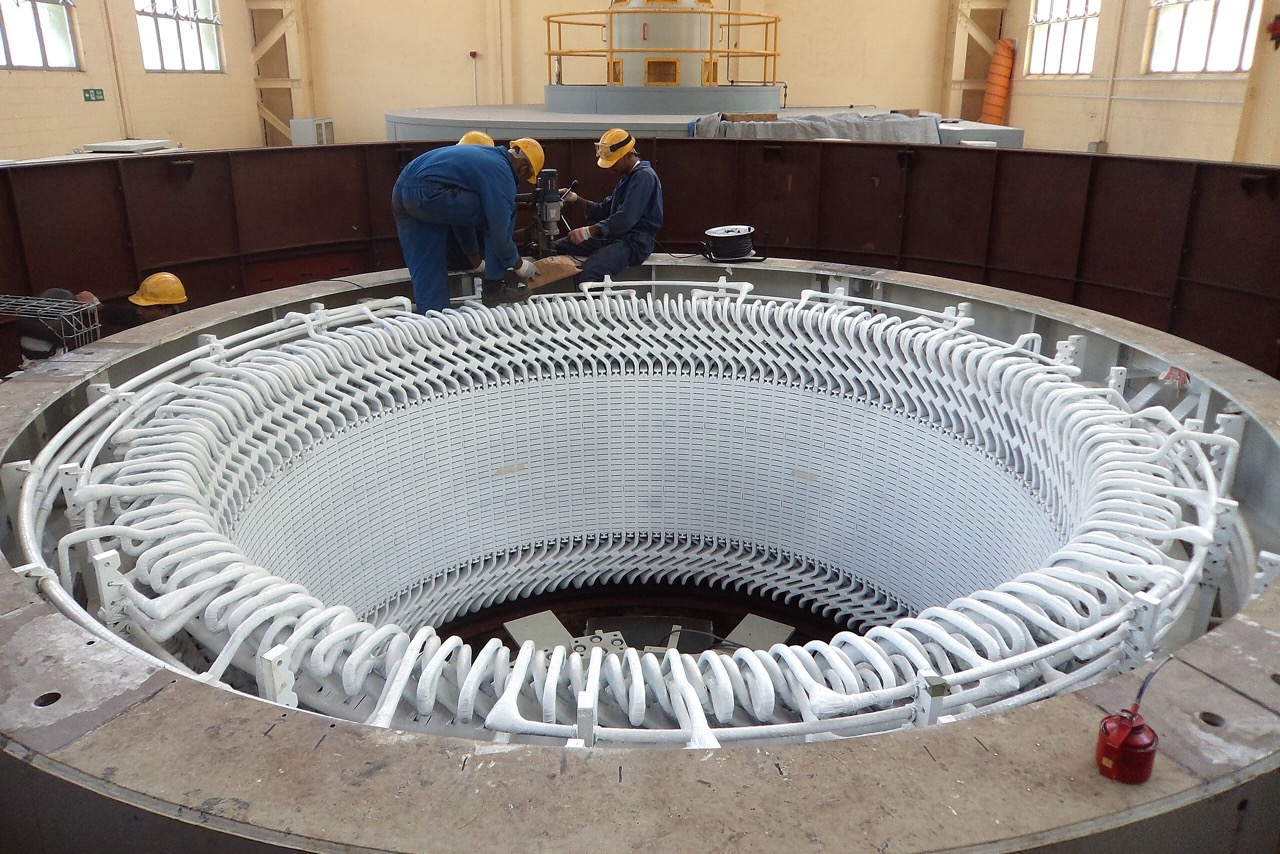
\includegraphics[width=0.9\textwidth]{fig/lec05/Stator_winding_at_WPS.jpg}
			\caption{Hydrogenerator with form-found stator winding (source: \href{https://commons.wikimedia.org/wiki/File:Stator_winding_at_WPS.JPG}{Wikimedia Commons},  	Astronomyinertia, \href{https://creativecommons.org/licenses/by-sa/3.0/deed.en}{CC~BY-SA~3.0})}
		\end{subfigure}
		\caption{Examples of three-phase stator windings with different configurations} 
        \label{fig:Stator_windings_examples}
	\end{figure}
\end{frame}

%%%%%%%%%%%%%%%%%%%%%%%%%%%%%%%%%%%%%%%%%%%%%%%%%%%%%%%%%%%%%
%% Winding as a distributed coil system %%
%%%%%%%%%%%%%%%%%%%%%%%%%%%%%%%%%%%%%%%%%%%%%%%%%%%%%%%%%%%%%
\begin{frame}
	\frametitle{Winding as a distributed coil system}
    In contrast to the lumped-coil representation from \figref{fig:Simple_three_phase_stator_lumped_coils}, the stator coils per phase are distributed over the stator circumference. To describe the winding layout, we (re-)introduce:
    \begin{gather*}
		Q: \mbox{number of slots}, \quad m: \mbox{number of phases (usually $m=3$)}, \\ q=\frac{Q}{2 p m}: \mbox{number of notches  (number of slots per phase and pole)}, \quad \rho_\mathrm{p}: \mbox{pole pitch (elec.).}
	\end{gather*}
    \begin{figure}
        \centering
        \includegraphics[width=0.8\textwidth]{fig/lec05/Scheme_distributed_winding.pdf}
        \caption{Example scheme of a distributed winding with $Q=18, p = 1, q=3$ (adapted from J.~B\"ocker, \textit{Controlled Three-Phase Drives}, Paderborn University, 2021)}
        \label{fig:Scheme_distributed_winding}
    \end{figure}
\end{frame}

%%%%%%%%%%%%%%%%%%%%%%%%%%%%%%%%%%%%%%%%%%%%%%%%%%%%%%%%%%%%%
%% Distributed winding: same width coils %%
%%%%%%%%%%%%%%%%%%%%%%%%%%%%%%%%%%%%%%%%%%%%%%%%%%%%%%%%%%%%%
\begin{frame}
	\frametitle{Distributed winding: same width coils}
    \begin{figure}
		\centering
		\begin{subfigure}[b]{0.49\textwidth}
			\centering
			\includegraphics[height=0.35\textheight]{fig/lec05/Distributed_winding_same_width_01.pdf}
			\caption{Simplified unwound cross-section view (adapted from J.~B\"ocker, \textit{Controlled Three-Phase Drives}, Paderborn University, 2021)}
		\end{subfigure}
		\hfill
		\begin{subfigure}[b]{0.49\textwidth}
			\centering
			\includegraphics[height=0.35\textheight]{fig/lec05/Distributed_winding_same_width_02.pdf}
			\caption{Front view on end winding  (adapted from W.~Novender, \textit{Elektrische Maschinen}, Technische Hochschule Mittelhessen, 2023)}
		\end{subfigure}
		\caption{Realization of a distributed winding through windings of same width $y$} 
        \label{fig:Distributed_winding_same_width}
	\end{figure}
\end{frame}

%%%%%%%%%%%%%%%%%%%%%%%%%%%%%%%%%%%%%%%%%%%%%%%%%%%%%%%%%%%%%
%% Distributed winding: varying width coils %%
%%%%%%%%%%%%%%%%%%%%%%%%%%%%%%%%%%%%%%%%%%%%%%%%%%%%%%%%%%%%%
\begin{frame}
	\frametitle{Distributed winding: varying width coils}
    \begin{figure}
		\centering
		\begin{subfigure}[b]{0.49\textwidth}
			\centering
			\includegraphics[height=0.35\textheight]{fig/lec05/Distributed_winding_different_width_01.pdf}
			\caption{Simplified unwound cross-section view (adapted from J.~B\"ocker, \textit{Controlled Three-Phase Drives}, Paderborn University, 2021)}
		\end{subfigure}
		\hfill
		\begin{subfigure}[b]{0.49\textwidth}
			\centering
			\includegraphics[height=0.35\textheight]{fig/lec05/Distributed_winding_different_width_02.pdf}
			\caption{Front view on end winding  (adapted from W.~Novender, \textit{Elektrische Maschinen}, Technische Hochschule Mittelhessen, 2023)}
		\end{subfigure}
		\caption{Realization of a distributed winding through windings of varying widths $y_i$} 
        \label{fig:Distributed_winding_different_width}
	\end{figure}
\end{frame}

%%%%%%%%%%%%%%%%%%%%%%%%%%%%%%%%%%%%%%%%%%%%%%%%%%%%%%%%%%%%%
%% Distribution factor %%
%%%%%%%%%%%%%%%%%%%%%%%%%%%%%%%%%%%%%%%%%%%%%%%%%%%%%%%%%%%%%
\begin{frame}
	\frametitle{Distribution factor}
    As a result of the winding distribution, the MMF results in a staircase form as shown in \figref{fig:Distributed_winding_MMF}. Hence, the field distribution calculation from \eqref{eq:B_single_phase_coil_fourier_series} has to be adapted. 
    \begin{figure}
        \centering
        \includegraphics[width=0.75\textwidth]{fig/lec05/Distributed_winding_MMF.pdf}
        \caption{Example of the MMF of a distributed winding scheme}
        \label{fig:Distributed_winding_MMF}
    \end{figure}
\end{frame}

%%%%%%%%%%%%%%%%%%%%%%%%%%%%%%%%%%%%%%%%%%%%%%%%%%%%%%%%%%%%%
%% Distribution factor (cont.)%%
%%%%%%%%%%%%%%%%%%%%%%%%%%%%%%%%%%%%%%%%%%%%%%%%%%%%%%%%%%%%%
\begin{frame}
	\frametitle{Distribution factor  (cont.)}
    \begin{columns}
		\begin{column}{0.6\textwidth}
	        Starting from
            \begin{align*}
                B_\mathrm{a}(\vartheta_\mathrm{el}) &= \sum_{k=1,3,5,\ldots}^{\infty} \hat{B}_{\mathrm{c}}^{(k)} \cos(k \vartheta_\mathrm{el})\\ \hat{B}_{\mathrm{c}}^{(k)} &= \frac{2}{\pi} \int_{-\pi/2}^{\pi/2} B(\vartheta_\mathrm{el}) \cos(k \vartheta_\mathrm{el}) \mathrm{d}\vartheta_\mathrm{el}
            \end{align*}
            \onslide<2->{%
                we rewrite the integral considering shifted coils by $\Delta \vartheta$ steps (i.e., $k \Delta \vartheta$ steps for the $k$-th harmonic order) with $N/q$ turns per coil based on the distribution of a single lumped coil $B'$ from \eqref{eq:B_single_phase_coil_fourier_series_coefficients}:
            \begin{equation*}
                \hat{B}_{\mathrm{c}}^{(k)} = \frac{2}{\pi q} \mathrm{Re}\left\{\sum_{l=0}^{q-1}e^{\mathrm{j} \Delta\vartheta_l k}\int_{-\pi/2}^{\pi/2} B'(\vartheta_\mathrm{el}) \cos(k \vartheta_\mathrm{el}) \mathrm{d}\vartheta_\mathrm{el}\right\}.
            \end{equation*}}
        \end{column}
        \begin{column}{0.4\textwidth}
            \begin{figure}
                \centering
                \includegraphics[width=0.9\textwidth]{fig/lec05/MMF_single_phase_distributed.pdf}
                \caption{Representation of the coil displacement by $\Delta \vartheta$ steps for a distributed winding with $q=3$ and $p=1$}
                \label{fig:MMF_single_phase_distributed}
            \end{figure}
        \end{column}
    \end{columns}
\end{frame}

%%%%%%%%%%%%%%%%%%%%%%%%%%%%%%%%%%%%%%%%%%%%%%%%%%%%%%%%%%%%%
%% Distribution factor (cont.)%%
%%%%%%%%%%%%%%%%%%%%%%%%%%%%%%%%%%%%%%%%%%%%%%%%%%%%%%%%%%%%%
\begin{frame}
	\frametitle{Distribution factor  (cont.)}
   The discrete coil displacement angles are (assuming that the $Q$ slots are evenly distributed over the stator circumference, i.e., $\Delta \vartheta = p 2  \pi/Q$)
   \begin{equation}
    \Delta\vartheta_l = -\frac{q-1}{2} \frac{\pi}{m q} + l \frac{\pi}{m q} = -\frac{q-1}{2} p \frac{2\pi}{Q} + l p \frac{2\pi}{Q} \quad \mbox{for } l=0,1,\ldots,q-1.
   \end{equation}\pause
   Hence, we can rewrite the Fourier series coefficient integral as:
   \begin{equation}
    \hat{B}_{\mathrm{c}}^{(k)} = \underbrace{\frac{1}{q}\mathrm{Re}\left\{\sum_{l=0}^{q-1} e^{\mathrm{j} \Delta\vartheta_l k}\right\} }_{\xi_{\mathrm{d},k}} \underbrace{\frac{2}{\pi}\int_{-\pi/2}^{\pi/2} B'(\vartheta_\mathrm{el}) \cos(k \vartheta_\mathrm{el}) \mathrm{d}\vartheta_\mathrm{el} \vphantom{\sum_{l=0}^{q-1}}}_{\mbox{single lumped-coil integral}}.
    \label{eq:B_single_phase_coil_fourier_series_coefficients_distributed}
\end{equation}
Hence, the Fourier coefficient of every harmonic order $k$ is multiplied by the distribution factor $\xi_{\mathrm{d},k}$. 
\end{frame}

%%%%%%%%%%%%%%%%%%%%%%%%%%%%%%%%%%%%%%%%%%%%%%%%%%%%%%%%%%%%%
%% Distribution factor (cont.)%%
%%%%%%%%%%%%%%%%%%%%%%%%%%%%%%%%%%%%%%%%%%%%%%%%%%%%%%%%%%%%%
\begin{frame}
	\frametitle{Distribution factor  (cont.)}
    \onslide<+->
    To write this $\xi_{\mathrm{d},k}$ more compactly, we rearrange 
    \begin{equation}
        \sum_{l=0}^{q-1} e^{\mathrm{j} \Delta\vartheta_l k} = \sum_{l=0}^{q-1} e^{\mathrm{j} k (-\frac{q-1}{2} p \frac{2\pi}{Q} + l p \frac{2\pi}{Q})} \uncover<+->{= e^{- \mathrm{j} k \frac{q-1}{2} p \frac{2\pi}{Q}} \sum_{l=0}^{q-1} \left(e^{\mathrm{j} k  p \frac{2\pi}{Q}}\right)^l}
        \label{eq:sum_exp_distribution_factor}
    \end{equation}
    \onslide<+->
    and utilize the finite geometric series expression
    $$
    \sum_{l=0}^{q-1} x^l = \frac{1-x^q}{1-x}
    $$
    \onslide<+->
    to rewrite
    $$
    \sum_{l=0}^{q-1} \left(e^{\mathrm{j} k  p \frac{2\pi}{Q}}\right)^l = \frac{1-e^{\mathrm{j} k q p \frac{2\pi}{Q}}}{1-e^{\mathrm{j} k  p \frac{2\pi}{Q}}}.
    $$
\end{frame}

%%%%%%%%%%%%%%%%%%%%%%%%%%%%%%%%%%%%%%%%%%%%%%%%%%%%%%%%%%%%%
%% Distribution factor (cont.)%%
%%%%%%%%%%%%%%%%%%%%%%%%%%%%%%%%%%%%%%%%%%%%%%%%%%%%%%%%%%%%%
\begin{frame}
	\frametitle{Distribution factor  (cont.)}
    \onslide<+->
    The latter can be further rewritten as
    $$
    \frac{1-e^{\mathrm{j} k q p\frac{2\pi}{Q}}}{1-e^{\mathrm{j} k p\frac{2\pi}{Q}}} = \frac{e^{\mathrm{j} k q p\frac{2\pi}{Q}\frac{1}{2}}\left(e^{-\mathrm{j} k q p\frac{2\pi}{Q}\frac{1}{2}}-e^{\mathrm{j} k q p\frac{2\pi}{Q}\frac{1}{2}}\right)}{e^{\mathrm{j} k p\frac{2\pi}{Q}\frac{1}{2}}\left(e^{-\mathrm{j} k p\frac{2\pi}{Q}\frac{1}{2}}-e^{\mathrm{j} k p\frac{2\pi}{Q}\frac{1}{2}}\right)}.
    $$
    \onslide<+->
    Utilizing the identity
    $$
    \sin(x) = \frac{e^{\mathrm{j} x}-e^{-\mathrm{j} x}}{2\mathrm{j}}
    $$
    \onslide<+->
    we can further rewrite
    \begin{equation}
        \uncover<+->{\sum_{l=0}^{q-1} \left(e^{\mathrm{j} k  p\frac{2\pi}{Q}}\right)^l =\frac{1-e^{\mathrm{j} k q p\frac{2\pi}{Q}}}{1-e^{\mathrm{j} k p\frac{2\pi}{Q}}} = \frac{e^{\mathrm{j} k q p\frac{2\pi}{Q}\frac{1}{2}}(-2\mathrm{j})\sin(k q p\frac{2\pi}{Q}\frac{1}{2})}{e^{\mathrm{j} k p\frac{2\pi}{Q}\frac{1}{2}}(-2\mathrm{j})\sin(k p\frac{2\pi}{Q}\frac{1}{2})}}\uncover<+->{=e^{\mathrm{j}k\frac{2 \pi}{Q}\frac{q-1}{2}}\frac{\sin(k q p\frac{2\pi}{Q}\frac{1}{2})}{\sin(k p\frac{2\pi}{Q}\frac{1}{2})}.}
        \label{eq:sum_exp_distribution_factor_simplified}
    \end{equation}
\end{frame}

%%%%%%%%%%%%%%%%%%%%%%%%%%%%%%%%%%%%%%%%%%%%%%%%%%%%%%%%%%%%%
%% Distribution factor (cont.)%%
%%%%%%%%%%%%%%%%%%%%%%%%%%%%%%%%%%%%%%%%%%%%%%%%%%%%%%%%%%%%%
\begin{frame}
	\frametitle{Distribution factor  (cont.)}
    \onslide<+->
    Inserting \eqref{eq:sum_exp_distribution_factor_simplified} into \eqref{eq:sum_exp_distribution_factor} we finally receive
    \begin{equation}
        \begin{split}
            \xi_{\mathrm{d},k} &= \frac{1}{q}\mathrm{Re}\left\{\sum_{l=0}^{q-1} e^{\mathrm{j} \Delta\vartheta_l k}\right\} = \frac{1}{q} e^{- \mathrm{j} k p\frac{2\pi}{Q} \frac{q-1}{2} } e^{\mathrm{j}k\frac{2 \pi}{Q}\frac{q-1}{2}}\frac{\sin(k q p\frac{2\pi}{Q}\frac{1}{2})}{\sin(k p\frac{2\pi}{Q}\frac{1}{2})}\\
            \uncover<+->{&= \frac{\sin(k q p\frac{2\pi}{Q}\frac{1}{2})}{q\sin(k p\frac{2\pi}{Q}\frac{1}{2})} = \frac{\sin(k q p \frac{\pi}{Q})}{q\sin(k p \frac{\pi}{Q})}}\\
            \uncover<+->{&= \frac{\sin\left(\frac{k \pi}{2 m}\right)}{q\sin\left(\frac{k \pi}{2 m q}\right)}.}
    \end{split}
    \end{equation}
    \begin{itemize}
        \item<+-> $|\xi_{\mathrm{d},k}| \leq 1$ holds for all parameter combinations.
        \item<+-> The factor describes the change of each harmonic component due to the distributed winding compared to the (idealized) lumped-coil case.
    \end{itemize}
\end{frame}

%%%%%%%%%%%%%%%%%%%%%%%%%%%%%%%%%%%%%%%%%%%%%%%%%%%%%%%%%%%%%
%% Pitch factor %%
%%%%%%%%%%%%%%%%%%%%%%%%%%%%%%%%%%%%%%%%%%%%%%%%%%%%%%%%%%%%%
\begin{frame}
	\frametitle{Pitch factor}
    \begin{columns}
		\begin{column}{0.6\textwidth}
	        If windings are not implemented as diametral winding, i.e., the winding width $y$ is smaller than the pole pitch $\rho_\mathrm{p}$, 
            $$y < \rho_\mathrm{p}=\pi,$$
            the winding is called chorded. \onslide<2->{Hence, the starting and end position of the coil are shifted towards $\pm(y/\rho_\mathrm{p})(\pi/2)$ along the circumference. Consequently, the Fourier coefficients of the chorded winding are:
            \begin{equation}
                \hat{B}_{\mathrm{c}}^{(k)} = \frac{2}{\pi} \int_{-\frac{\pi}{2}\frac{y}{\rho_\mathrm{p}}}^{\frac{\pi}{2}\frac{y}{\rho_\mathrm{p}}} B(\vartheta_\mathrm{el}) \cos(k \vartheta_\mathrm{el}) \mathrm{d}\vartheta_\mathrm{el}.
                \label{eq:Pitch_factor_fourier_coefficients}
            \end{equation}}
        \end{column}
        \begin{column}{0.4\textwidth}
            \begin{figure}
                \centering
                \includegraphics[width=0.9\textwidth]{fig/lec05/Single_phase_chording.pdf}
                \caption{Representation of a chorded coil for a distributed winding with $q=3$ and $p=1$}
                \label{fig:Single_phase_chording}
            \end{figure}
        \end{column}
    \end{columns}
\end{frame}

%%%%%%%%%%%%%%%%%%%%%%%%%%%%%%%%%%%%%%%%%%%%%%%%%%%%%%%%%%%%%
%% Pitch factor (cont.) %%
%%%%%%%%%%%%%%%%%%%%%%%%%%%%%%%%%%%%%%%%%%%%%%%%%%%%%%%%%%%%%
\begin{frame}
	\frametitle{Pitch factor (cont.)}
    \onslide<+->
    Continuing from \eqref{eq:Pitch_factor_fourier_coefficients}, we can rewrite the integral as
    \begin{equation}
        \begin{split}
            \hat{B}_{\mathrm{c}}^{(k)} &= \frac{2}{\pi} \int_{-\frac{\pi}{2}\frac{y}{\rho_\mathrm{p}}}^{\frac{\pi}{2}\frac{y}{\rho_\mathrm{p}}} B(\vartheta_\mathrm{el}) \cos(k \vartheta_\mathrm{el}) \mathrm{d}\vartheta_\mathrm{el} \uncover<+->{= \frac{2}{\pi}\hat{B}\cos(\omega t) \int_{-\frac{\pi}{2}\frac{y}{\rho_\mathrm{p}}}^{\frac{\pi}{2}\frac{y}{\rho_\mathrm{p}}} \cos(k \vartheta_\mathrm{el}) \mathrm{d}\vartheta_\mathrm{el}}\\
            \uncover<+->{&= \frac{2}{\pi}\hat{B}\cos(\omega t)\frac{1}{k} \left[\sin(k\frac{\pi}{2}\frac{y}{\rho_\mathrm{p}}) - \sin(-k\frac{\pi}{2}\frac{y}{\rho_\mathrm{p}})\right]}\uncover<+->{ = \frac{4}{\pi}\hat{B}\cos(\omega t)\frac{1}{k} \sin(k\frac{\pi}{2}\frac{y}{\rho_\mathrm{p}}).}
        \end{split}
        \label{eq:Pitch_factor_fourier_coefficients_rewritten} 
    \end{equation}
    \onslide<+->
    Compared to the unchored case \eqref{eq:B_single_phase_coil_fourier_series_coefficients}, the Fourier coefficients are
    $$\frac{\sin\left(k\frac{\pi}{2}\frac{y}{\rho_\mathrm{p}}\right)}{\sin\left(k\frac{\pi}{2}\right)}$$ smaller. \onslide<+-> As the magnitude of the denominator is always one, we define
    \begin{equation}
        \xi_{\mathrm{p},k} = \sin\left(k\frac{\pi}{2}\frac{y}{\rho_\mathrm{p}}\right)
        \label{eq:Pitch_factor_definition}
    \end{equation} 
    as the pitch factor.
\end{frame}

%%%%%%%%%%%%%%%%%%%%%%%%%%%%%%%%%%%%%%%%%%%%%%%%%%%%%%%%%%%%%
%% Winding factor %%
%%%%%%%%%%%%%%%%%%%%%%%%%%%%%%%%%%%%%%%%%%%%%%%%%%%%%%%%%%%%%
\begin{frame}
	\frametitle{Winding factor}
    \onslide<+->
    Considering both, a distributed and chorded winding, we receive
    \begin{equation}
        \begin{split}
            \hat{B}_{\mathrm{c}}^{(k)} &= \frac{1}{q}\mathrm{Re}\left\{\sum_{l=0}^{q-1} e^{\mathrm{j} \Delta\vartheta_l k}\right\}  \frac{2}{\pi}\int_{-\frac{\pi}{2}\frac{y}{\rho_\mathrm{p}}}^{\frac{\pi}{2}\frac{y}{\rho_\mathrm{p}}} B(\vartheta_\mathrm{el}) \cos(k \vartheta_\mathrm{el}) \mathrm{d}\vartheta_\mathrm{el}\\\uncover<+->{
            &=\cdots\\
            &= \frac{4}{\pi}\hat{B}\cos(\omega t)\frac{1}{k} \sin\left(k\frac{\pi}{2}\frac{y}{\rho_\mathrm{p}}\right)  \frac{\sin\left(\frac{k \pi}{2 m}\right)}{q\sin\left(\frac{k \pi}{2 m q}\right)}\\}
            \uncover<+->{&= \frac{4}{\pi}\hat{B}\cos(\omega t)\frac{1}{k} \underbrace{\xi_{\mathrm{d},k} \xi_{\mathrm{p},k}}_{\xi_{\mathrm{w},k}}}
            \end{split}
        \label{eq:Winding_factor_fourier_coefficients} 
    \end{equation}
    \onslide<3->
    with $\xi_{\mathrm{w},k} = \xi_{\mathrm{d},k} \xi_{\mathrm{p},k}$ being the winding factor. \onslide<+-> It describes the change of each harmonic component due to the distributed and chorded winding compared to the (idealized) lumped-coil case (which would be equivalent to $\xi_{\mathrm{w},k}=1$).
\end{frame}

%%%%%%%%%%%%%%%%%%%%%%%%%%%%%%%%%%%%%%%%%%%%%%%%%%%%%%%%%%%%%
%% Winding factor:examples %%
%%%%%%%%%%%%%%%%%%%%%%%%%%%%%%%%%%%%%%%%%%%%%%%%%%%%%%%%%%%%%
\begin{frame}
	\frametitle{Winding factor: examples}
    \begin{table}
        \centering
        \begin{tabular}{r c c c c c c c c c}
            & \multicolumn{3}{c}{Machine A} & \multicolumn{3}{c}{Machine B} & \multicolumn{3}{c}{Machine C}\\
            \toprule
            & \multicolumn{3}{c}{$q=1, \quad y/\rho_\mathrm{p}=2/3,$} & \multicolumn{3}{c}{$q=2, \quad y/\rho_\mathrm{p}=5/6,$} & \multicolumn{3}{c}{$q=3, \quad y/\rho_\mathrm{p}=7/9,$}\\
            & \multicolumn{3}{c}{$Q/p = 6$} & \multicolumn{3}{c}{$Q/p = 12$} &\multicolumn{3}{c}{$Q/p = 18$}\\
            \cmidrule{2-10}
            $k$ & $\xi_{\mathrm{d},k}$ & $\xi_{\mathrm{p},k}$ & $\xi_{\mathrm{w},k}$ & $\xi_{\mathrm{d},k}$ & $\xi_{\mathrm{p},k}$ & $\xi_{\mathrm{w},k}$ & $\xi_{\mathrm{d},k}$ & $\xi_{\mathrm{p},k}$ & $\xi_{\mathrm{w},k}$\\
            \midrule
            1 & 1 & 0.866 & 0.866 & 0.966 & 0.966 & 0.933 & 0.960 & 0.940 & 0.902\\
            3 & 1 & 0 & 0 & 0.707 & -0.707 & -0.500 & 0.667 & -0.500 & -0.333\\
            5 & 1 & -0.866 & -0.866 & 0.259 & 0.259 & 0.067 & 0.218 & -0.174 & -0.038\\
            7 & 1 & 0.866 & 0.866 & -0.259 & 0.259 & -0.067 & -0.177 & 0.766 & -0.136\\
            9 & 1 & 0 & 0 & -0.707 & -0.707 & 0.500 & -0.333 & -1.000 & 0.333\\
            11 & 1 & -0.866 & -0.866 & -0.966 & 0.966 & -0.933 & -0.177 & 0.776 & -0.136\\
            13 & 1 & 0.866 & 0.866 & -0.966 & -0.966 & 0.933 & 0.218 & -0.174 & -0.038\\
            15 & 1 & 0 & 0 & -0.707 & 0.707 & -0.500 & 0.667 & -0.500 & -0.333\\
            \bottomrule
        \end{tabular}
        \caption{Winding factors for different winding configurations for three-phase machines ($m=3$)}
        \label{tab:Winding_factors}
    \end{table}
\end{frame}

%%%%%%%%%%%%%%%%%%%%%%%%%%%%%%%%%%%%%%%%%%%%%%%%%%%%%%%%%%%%%
%% Winding factor: remarks %%
%%%%%%%%%%%%%%%%%%%%%%%%%%%%%%%%%%%%%%%%%%%%%%%%%%%%%%%%%%%%%
\begin{frame}
	\frametitle{Winding factor: remarks}
    \begin{varblock}{Winding factor interpretation}
        The winding factor $\xi_{\mathrm{w},k}$ mathematically maps a (real-world) distributed (and eventually chorded) winding with $N$ turns in slots distributed over the stator circumference to an idealized (abstract) lumped-coil representation with $N \cdot \xi_{\mathrm{w},k}$ (effective) turns. For following calculation steps (e.g., in a three-phase machine model -- compare \figref{fig:Simple_three_phase_stator_lumped_coils}), one can utilize the simplified lumped-coil representation without systematic modeling errors thanks to the winding factor concept.
    \end{varblock}
    \begin{itemize}
        \item<2-> With respect to \tabref{tab:Winding_factors} one can also observe that the winding configuration choice has a direct impact on the harmonic content of the flux density distribution.
        \item<3-> As those will also influence the production of torque and induced voltage (harmonics), the winding factor is a crucial parameter for the design of electrical machines.
    \end{itemize}
\end{frame}

%%%%%%%%%%%%%%%%%%%%%%%%%%%%%%%%%%%%%%%%%%%%%%%%%%%%%%%%%%%%%
%% Winding factor: limitations %%
%%%%%%%%%%%%%%%%%%%%%%%%%%%%%%%%%%%%%%%%%%%%%%%%%%%%%%%%%%%%%
\begin{frame}
	\frametitle{Winding factor: limitations}
    \onslide<+->
    The winding factor approach leading to \eqref{eq:Winding_factor_fourier_coefficients} was based on several (implicit) assumptions:
    \begin{itemize}
        \item<+-> The number of slots per phase and pole is a (positive) integer: $q \in \mathbb{N}$.
        \item<+-> The slot distribution is even over the stator circumference.
    \end{itemize}
    \onslide<+->
    However, these assumptions do not apply to all (typical) winding configurations, in particular fractional slot windings where $$q=\frac{Q}{2 p m} \in \mathbb{Q}$$ is represented by a common fraction, i.e., rational number. 
    \begin{figure}
        \centering
        \includegraphics[width=0.75\textwidth]{fig/lec05/Fractional_slot_concentrated_winding_example.pdf}
        \caption{Example scheme of a fractional slot concentrated winding with $Q=9$, $p = 3$, $q=1/2$ (adapted from J.~B\"ocker, \textit{Controlled Three-Phase Drives}, Paderborn University, 2021)}
        \label{fig:Fractional_slot_concentrated_winding_example}
    \end{figure}
\end{frame}

%%%%%%%%%%%%%%%%%%%%%%%%%%%%%%%%%%%%%%%%%%%%%%%%%%%%%%%%%%%%%
%% Concentrated winding %%
%%%%%%%%%%%%%%%%%%%%%%%%%%%%%%%%%%%%%%%%%%%%%%%%%%%%%%%%%%%%%
\begin{frame}
	\frametitle{Concentrated winding}
    \begin{itemize}
        \item Concentrated winding: the coils per phase are wound around single stator teeth.
        \item Allows for smaller end windings (i.e., less copper and reduced motor length) compared to distributed windings.
    \end{itemize}
    \begin{figure}
		\begin{columns}
			\begin{column}{0.4\textwidth}
					\centering
					\includegraphics[width=0.9\textwidth]{fig/lec05/Concentrated_winding_example.jpg}
			\end{column}
			\begin{column}{0.6\textwidth}
				\caption{\raggedright Example of a concentrated winding where conductors form coils centered around single stator teeth (source:  Chan-Ho Baek et al., \textit{Iron Loss Analysis of a Concentrated Winding Type Interior Permanent Magnet Synchronous Motor with Single and Dual Layer Magnet Shape}, MDPI Machines, 2021, \href{https://creativecommons.org/licenses/by/4.0/}{CC BY 4.0})}
				\label{fig:Concentrated_winding_example}
			\end{column}
		\end{columns}
	\end{figure}
\end{frame}


%%%%%%%%%%%%%%%%%%%%%%%%%%%%%%%%%%%%%%%%%%%%%%%%%%%%%%%%%%%%%
%% Complex winding factor %%
%%%%%%%%%%%%%%%%%%%%%%%%%%%%%%%%%%%%%%%%%%%%%%%%%%%%%%%%%%%%%
\begin{frame}
	\frametitle{Complex winding factor}
    \onslide<+->
    The complex winding factor (here: for phase a) is defined as
    \begin{equation}
        \underline{\xi}_{\mathrm{a},k} = \frac{1}{\mathrm{j}N_\mathrm{a}}\sum_{i=1}^{Q} N_{\mathrm{a},i}e^{\mathrm{j}k\vartheta_{\mathrm{el},\mathrm{a},i}}
        \label{eq:Complex_winding_factor_definition}
    \end{equation} 
    with $N_{\mathrm{a},i}\in \mathbb{Z}$ being the number of conductors in slot $i$ at the position $\vartheta_{\mathrm{el},\mathrm{a},i}$ \onslide<+-> with 
    \begin{equation}
        N_\mathrm{a} = \sum_{i=1}^{Q} |N_{\mathrm{a},i}|
        \label{eq:Complex_winding_factor_total_number_conductors}
    \end{equation}
    being the total number of conductors. \onslide<+-> Moreover, $N_{\mathrm{a},i}$ represents the orientation of each conductor by
    \begin{itemize}
        \item $N_{\mathrm{a},i} = 0$: no conductor is in slot $i$,
        \item<+-> $N_{\mathrm{a},i} >0 $: conductor is oriented towards the positive $z$-axis (directed towards reader),
        \item<+-> $N_{\mathrm{a},i} <0 $: conductor is oriented towards the negative $z$-axis (directed away from reader).
    \end{itemize}
\end{frame}

%%%%%%%%%%%%%%%%%%%%%%%%%%%%%%%%%%%%%%%%%%%%%%%%%%%%%%%%%%%%%
%% Complex winding factor (cont.) %%
%%%%%%%%%%%%%%%%%%%%%%%%%%%%%%%%%%%%%%%%%%%%%%%%%%%%%%%%%%%%%
\begin{frame}
	\frametitle{Complex winding factor (cont.)}
    \onslide<1->
    The complex winding factor is a generalization of \eqref{eq:B_single_phase_coil_fourier_series_coefficients_distributed} weighting the contribution of each conductor to the $k$-th harmonic (compare \figref{fig:Representation_complex_winding_factor}). \onslide<2->Hence,
    \begin{itemize}
        \item<2-> the conductor positions $\vartheta_{\mathrm{el},\mathrm{a},i}$ are arbitrary and do not need to follow a specific distribution pattern (i.e., applicable to arbitrary slot configurations),
        \item<3-> the magnitude of the complex winding factor $|\underline{\xi}_{\mathrm{a},k}|\in[0,1]$ indicates the dampening of the harmonic component $k$ due to the winding configuration,
        \item<4-> the phase of the complex winding factor $\angle \underline{\xi}_{\mathrm{a},k}$ indicates the phase shift of the harmonic component $k$ compared to the winding layout. 
    \end{itemize}
    \onslide<1->
    \begin{figure}
        \centering
        \includegraphics[width=0.7\textwidth]{fig/lec05/Representation_complex_winding_factor.pdf}
        \caption{Qualitative illustration of the complex winding factor as a comparison of the actual current distribution compared to the ideal distribution belonging to a certain flux harmonic}
        \label{fig:Representation_complex_winding_factor}
    \end{figure}
\end{frame}

%%%%%%%%%%%%%%%%%%%%%%%%%%%%%%%%%%%%%%%%%%%%%%%%%%%%%%%%%%%%%
%% Complex winding factor (cont.) %%
%%%%%%%%%%%%%%%%%%%%%%%%%%%%%%%%%%%%%%%%%%%%%%%%%%%%%%%%%%%%%
\begin{frame}
	\frametitle{Complex winding factor (cont.)}
    While \eqref{eq:Complex_winding_factor_definition} represents the complex winding factor for phase a, the complex winding factor for phase b and c can be derived by rotating the coordinate system by $\pm 2\pi/3$:
    \begin{equation}
        \underline{\xi}_{\mathrm{b},k} = \frac{1}{\mathrm{j}N_\mathrm{b}}\sum_{i=1}^{Q} N_{\mathrm{b},i}e^{\mathrm{j}k\left(\vartheta_{\mathrm{el},\mathrm{a},i}+\frac{2\pi}{3}\right)}, \qquad  \underline{\xi}_{\mathrm{c},k} = \frac{1}{\mathrm{j}N_\mathrm{c}}\sum_{i=1}^{Q} N_{\mathrm{c},i}e^{\mathrm{j}k\left(\vartheta_{\mathrm{el},\mathrm{a},i}-\frac{2\pi}{3}\right)}.
        \label{eq:Complex_winding_factor_definition_phase_bc}    
    \end{equation}
    \pause
    Hence,
    \begin{equation}
        \underline{\xi}_{\mathrm{a},k} = e^{-\mathrm{j}k\frac{2\pi}{3}}\underline{\xi}_{\mathrm{b},k} = e^{\mathrm{j}k\frac{2\pi}{3}}\underline{\xi}_{\mathrm{c},k}
        \label{eq:Complex_winding_factor_relation}
    \end{equation}
    applies. 
    \pause
    \begin{varblock}{Harmonic orders}
        While regular symmetrical windings with $q\in\mathbb{N}$ will only produce certain harmonic orders ($k=1,3,5,7,\ldots$ -- cf. \eqref{eq:B_three_phase_stator_coil_fourier_series}), arbitrary winding configurations can produce further harmonic orders $k\in\mathbb{Q}$ (in particular if $q$ is a common fraction).
    \end{varblock}
\end{frame}

%%%%%%%%%%%%%%%%%%%%%%%%%%%%%%%%%%%%%%%%%%%%%%%%%%%%%%%%%%%%%
%% Complex winding factor (cont.) %%
%%%%%%%%%%%%%%%%%%%%%%%%%%%%%%%%%%%%%%%%%%%%%%%%%%%%%%%%%%%%%
\begin{frame}
	\frametitle{Complex winding factor: example}
    Based on the below table describing the winding scheme information from \figref{fig:Fractional_slot_concentrated_winding_example} we have
    \begin{align*}
        \underline{\xi}_{\mathrm{a},k} &= \frac{1}{\mathrm{j}6}\left(-1e^{\mathrm{j}\frac{k\pi}{3}} + 1 e^{\mathrm{j}\frac{k5\pi}{3}}-e^{\mathrm{j}\frac{k7\pi}{3}} + e^{\mathrm{j}\frac{k11\pi}{3}} - e^{\mathrm{j}\frac{k13\pi}{3}}+e^{\mathrm{j}\frac{k17\pi}{3}}\right),\\
        \underline{\xi}_{\mathrm{a},1} &= \frac{1}{\mathrm{j}6}\left(-1e^{\mathrm{j}\frac{\pi}{3}} + 1 e^{\mathrm{j}\frac{5\pi}{3}}-e^{\mathrm{j}\frac{7\pi}{3}} + e^{\mathrm{j}\frac{11\pi}{3}} - e^{\mathrm{j}\frac{13\pi}{3}}+e^{\mathrm{j}\frac{17\pi}{3}}\right) = -0.866,\\
        \underline{\xi}_{\mathrm{a},2} &= \frac{1}{\mathrm{j}6}\left(-1e^{\mathrm{j}\frac{2\pi}{3}} + 1 e^{\mathrm{j}\frac{10\pi}{3}}-e^{\mathrm{j}\frac{14\pi}{3}} + e^{\mathrm{j}\frac{22\pi}{3}} - e^{\mathrm{j}\frac{26\pi}{3}}+e^{\mathrm{j}\frac{34\pi}{3}}\right) = -0.866,\\
        \underline{\xi}_{\mathrm{a},3} &= \frac{1}{\mathrm{j}6}\left(-1e^{\mathrm{j}\pi} + 1 e^{\mathrm{j}5\pi}-e^{\mathrm{j}7\pi} + e^{\mathrm{j}11\pi} - e^{\mathrm{j}13\pi}+e^{\mathrm{j}17\pi}\right) = 0.
    \end{align*}
    \vspace{-0.35cm}
    \begin{table}
        \centering
        \begin{tabular}{l c c c c c c c c c}
            \toprule
           $i$-th slot & 1 & 2 & 3 & 4 & 5 & 6 & 7 & 8 & 9 \\ 
           $\vartheta_{\mathrm{el},\mathrm{a},i}$ & $\frac{1}{3}\pi$ & $\pi$ & $\frac{5}{3}\pi$ & $\frac{7}{3}\pi$ & $3\pi$ & $\frac{11}{3}\pi$ & $\frac{13}{3}\pi$ & $5\pi$ & $\frac{17}{3}\pi$\\ 
           \midrule
              $N_{\mathrm{a},i}$ & -1 & 0 & 1 & -1 & 0 & 1 & -1 & 0 & 1\\
              $N_{\mathrm{b},i}$ & 1 & -1 & 0 & 1 & -1 & 0 & 1 & -1 & 0\\
                $N_{\mathrm{c},i}$ & 0 & 1 & -1 & 0 & 1 & -1 & 0 & 1 & -1\\
            \bottomrule
        \end{tabular}
    \end{table}
\end{frame}